\documentclass[tikz, border=10pt]{standalone}
\usepackage[T1]{fontenc}
\usepackage{tikz}
\usetikzlibrary{shapes.geometric, arrows.meta, positioning}

\begin{document}
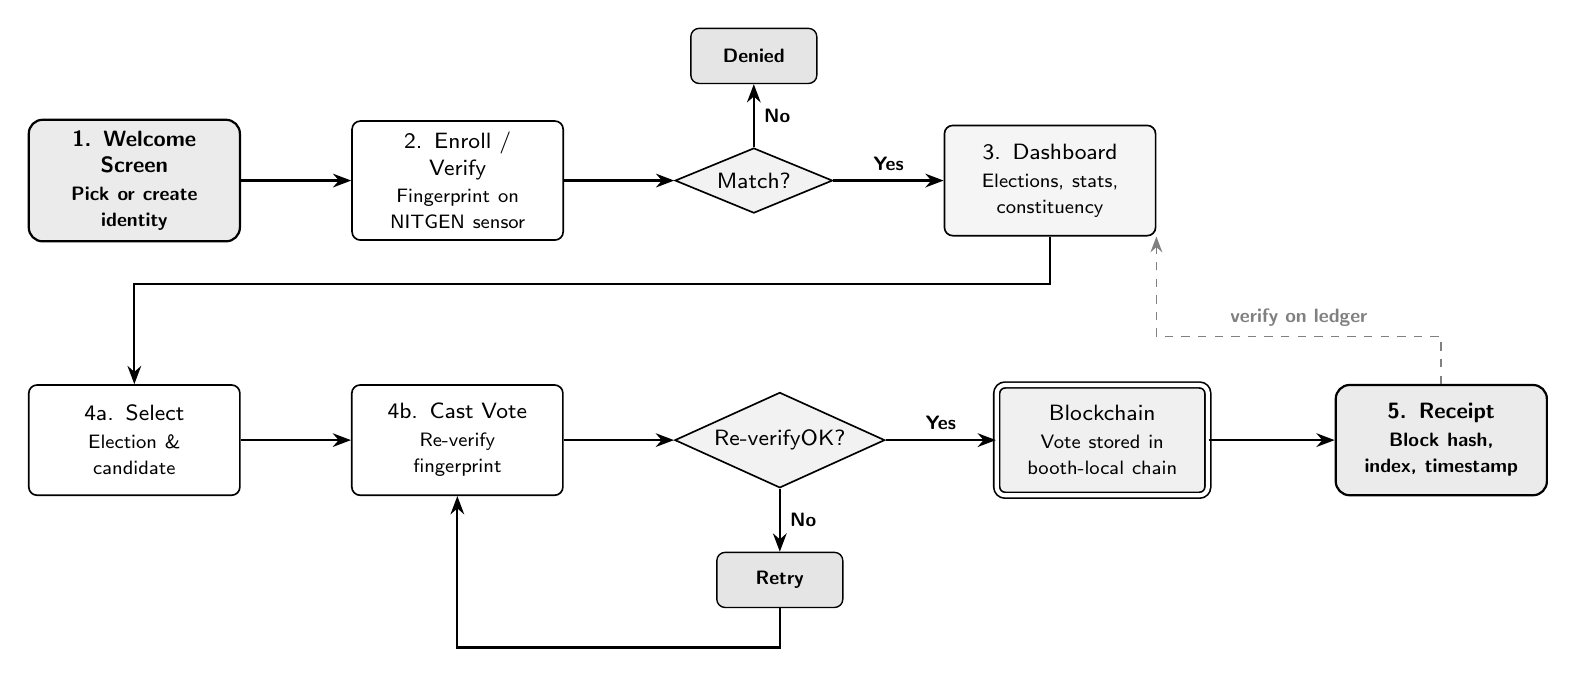
\begin{tikzpicture}[
    % ── Global ──
    node distance=1.6cm and 1.4cm,
    % ── Node Styles (print-friendly: high contrast, solid fills) ──
    startend/.style={
        rectangle, rounded corners=5pt,
        minimum width=2.6cm, minimum height=1.4cm,
        text centered, draw=black, line width=0.8pt,
        fill=black!8, font=\sffamily\footnotesize\bfseries,
        text width=2.4cm, inner sep=4pt
    },
    stepbox/.style={
        rectangle, rounded corners=3pt,
        minimum width=2.6cm, minimum height=1.4cm,
        text centered, draw=black, line width=0.6pt,
        fill=white, font=\sffamily\footnotesize,
        text width=2.4cm, inner sep=4pt
    },
    decision/.style={
        diamond, aspect=2.2,
        minimum width=2cm,
        text centered, draw=black, line width=0.6pt,
        fill=black!5, font=\sffamily\footnotesize,
        inner sep=2pt
    },
    databox/.style={
        rectangle, rounded corners=3pt,
        minimum width=2.6cm, minimum height=1.4cm,
        text centered, draw=black, line width=0.6pt,
        fill=black!6, font=\sffamily\footnotesize,
        text width=2.4cm, inner sep=4pt,
        double, double distance=1.5pt
    },
    rejected/.style={
        rectangle, rounded corners=3pt,
        minimum width=1.6cm, minimum height=0.7cm,
        text centered, draw=black, line width=0.5pt,
        fill=black!10, font=\sffamily\scriptsize\bfseries
    },
    arrow/.style={-Stealth, line width=0.8pt, draw=black},
    lbl/.style={font=\sffamily\scriptsize\bfseries},
]

% ════════════════════════════════════════════════════════
%  ROW 1: Steps 1 → 2 → Decision → 3
% ════════════════════════════════════════════════════════

\node (S1) [startend]
    {1. Welcome\\Screen\\[2pt]{\scriptsize Pick or create\\identity}};

\node (S2) [stepbox, right=of S1]
    {2. Enroll /\\Verify\\[2pt]{\scriptsize Fingerprint on\\NITGEN sensor}};

\node (D1) [decision, right=of S2]
    {Match?};

\node (D1no) [rejected, above=0.8cm of D1] {Denied};

\node (S3) [stepbox, right=of D1, fill=black!4]
    {3. Dashboard\\[2pt]{\scriptsize Elections, stats,\\constituency}};

% ════════════════════════════════════════════════════════
%  ROW 2: Steps 4a → 4b → Decision → Blockchain → 5
% ════════════════════════════════════════════════════════

\node (S4a) [stepbox, below=1.8cm of S1]
    {4a. Select\\[2pt]{\scriptsize Election \&\\candidate}};

\node (S4b) [stepbox, right=of S4a]
    {4b. Cast Vote\\[2pt]{\scriptsize Re-verify\\fingerprint}};

\node (D2) [decision, right=of S4b]
    {Re-verify\\OK?};

\node (D2no) [rejected, below=0.8cm of D2] {Retry};

\node (S4c) [databox, right=of D2]
    {Blockchain\\[2pt]{\scriptsize Vote stored in\\booth-local chain}};

\node (S5) [startend, right=1.6cm of S4c]
    {5. Receipt\\[2pt]{\scriptsize Block hash,\\index, timestamp}};

% ════════════════════════════════════════════════════════
%  ARROWS
% ════════════════════════════════════════════════════════

% Row 1
\draw [arrow] (S1)  -- (S2);
\draw [arrow] (S2)  -- (D1);
\draw [arrow] (D1)  -- node[lbl, above] {Yes} (S3);
\draw [arrow] (D1)  -- node[lbl, right] {No}  (D1no);

% Row 1 → Row 2 connector
\draw [arrow] (S3.south) -- ++(0,-0.6) -| (S4a.north);

% Row 2
\draw [arrow] (S4a) -- (S4b);
\draw [arrow] (S4b) -- (D2);
\draw [arrow] (D2)  -- node[lbl, above] {Yes} (S4c);
\draw [arrow] (D2)  -- node[lbl, right] {No}  (D2no);
\draw [arrow] (S4c) -- (S5);

% Retry loop — routed below the row to avoid overlap
\draw [arrow] (D2no.south) -- ++(0, -0.5) -| (S4b.south);

% Verify-on-ledger feedback (dashed)
\draw [-Stealth, dashed, line width=0.6pt, draw=black!50]
    (S5.north) -- ++(0, 0.6)
    -| node[lbl, near start, above, text=black!50] {\scriptsize verify on ledger} (S3.south east);

\end{tikzpicture}
\end{document}
